\subsection{Progettazione Concettuale}

Riassumendo l'analisi dei requisiti fatta precedentemente, si è giunti alla conclusione
che per modellare il nostro progetto avremo bisogno di:
\begin{itemize}
	
	\item una classe Country che rappresenta il concetto astratto di paese.
		Tale classe si specializza in 3 sotto-classi:	
		\begin{itemize}
			\item Nation;
			\item Continent;
			\item World.
		\end{itemize}
	
	\item una classe Confederation che rappresenta il concetto astratto di confederazione calcistica.
		Tale classe si specializza in 3 sotto-classi:	
		\begin{itemize}
			\item National Confederation;
			\item Continent Confederation;
			\item World Confederation.
		\end{itemize}

	\item una classe Competition che rappresenta il concetto astratto di competizione calcistica.
		Tale classe si specializza in 2 sotto classi:	
		\begin{itemize}
			\item Club Competition;
			\item National Competition.
		\end{itemize}	
		Ciascuna di queste sotto-classi si specializza poi in base al format in:
		\begin{itemize}
			\item League;
			\item Cup;
			\item Super Cup.
		\end{itemize}

	\item una classe Competition Edition che rappresenta il concetto astratto di
		edizione di una competizione calcistica.
	
	\item una classe Team che rappresenta il concetto astratto di squadra di calcio.
		Tale classe si specializza in 2 sotto-classi:
		\begin{itemize}
			\item Club Team;
			\item National Team.
		\end{itemize}	

	\item una classe Trophy che rappresenta il concetto astratto di trofeo calcistico.
		Tale classe si specializza in 2 sotto-classi:
		\begin{itemize}
			\item Player Trophy;
			\item Team Trophy.
		\end{itemize}

	\item una classe Prize che rappresenta il concetto astratto di premio calcistico.
		Tale classe si specializza in 2 sotto-classi:	
		\begin{itemize}
			\item Player Prize;
			\item Team Prize.
		\end{itemize}	

	\item una classe Player che rappresenta il concetto astratto di calciatore.

	\item una classe Position che rappresenta il concetto astratto di posizione di gioco.

	\item una classe Tag che rappresenta il concetto astratto di tag che si può assegnare
		ad un calciatore.

	\item una classe AttributeMental che rappresenta il concetto astratto di insieme di
		attributi che descrivono le caratteristiche mentali di un calciatore.
			
	\item una classe AttributePhysical che rappresenta il concetto astratto di insieme di
		attributi che descrivono le caratteristiche fisiche di un calciatore.
	
	\item una classe AttributeTechnical che rappresenta il concetto astratto di insieme di
		attributi che descrivono le caratteristiche tecniche di un calciatore.
	
	\item una classe AttributeGoalkeeping che rappresenta il concetto astratto di insieme di
		attributi che descrivono le caratteristiche di un portiere.

	\item una classe StatisticGeneral che rappresenta il concetto astratto di insieme di
		statistiche associabili al gioco di un calciatore.
		
	\item una classe StatisticGoalkeeper che rappresenta il concetto astratto di insieme di
		statistiche associabili al gioco di un portiere.

	\item una classe User Account che rappresenta il concetto astratto di utente dell'applicativo
		connesso al DataBase.
		
\end{itemize}

Sottolineiamo che abbiamo dato solo una descrizione concettuale delle principali classi
implementate senza dare una descrizione accurata degli attirbuti associati e senza approfondire
tutte le ulteriori classi associative ed associazioni che saranno chiaramente descritte
in modo schematico nei diagrammi UML e poi affrontate in modo approfondito nel dizionario
delle associazioni e nella documentazione interna al codice.
\newpage
\subsection{Class Diagram non ristrutturato}

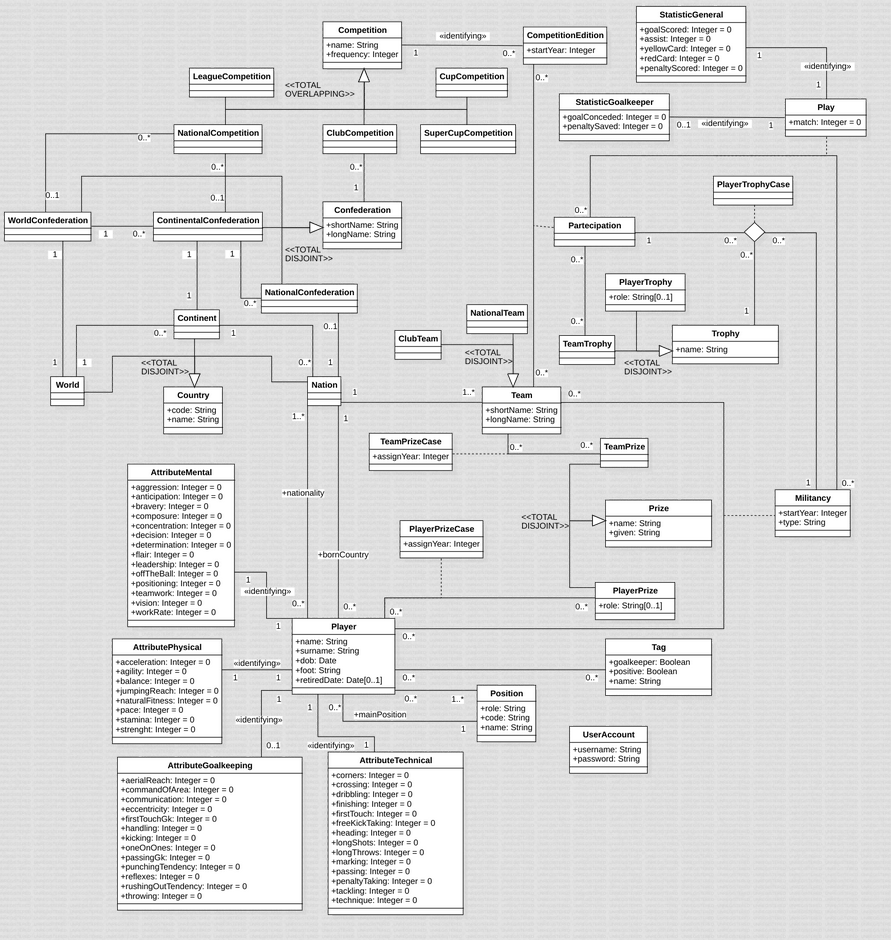
\includegraphics[width=\textwidth]{res/DOC_DATABASE/class_diagram_not_ristr}
\newpage

\subsection{Ristrutturazione del Class Diagram}

\subsubsection{Analisi delle Ridondanze}

\textbf{Classe: CompetitionEdition}

Si è scelto di  aggiungere un attributo che rappresenti l'anno di fine di una edizione di una
competizione calcistica per semplificare le viste sul DataBase, in quanto altrimenti sarebbe
stato necessario andare a valutare ogni volta il tipo di squadra della competizione associata.

Esempi di alcune operazioni svolte nel DataBase che coinvolgono l'anno di fine di un'edizione
di una competizione calcistica:
\begin{itemize}
	\item Mostrare le informazioni relative al gioco di un calciatore;
	\item Mostrare le informazioni relative all'edizione di una competizione calcistica.
\end{itemize}

\textbf{Classe: Player}

Supponendo un'alta frequenza di operazioni riguardanti i calciatori, e nello specifico in relazione
ai ruoli dei calciatori, si è deciso di introdurre nella classe Player un attributo ridondante
che rappresenti l'insieme dei ruoli del calciatore stesso.

L'alternativa sarebbe stata quella di andare a calcolare l'insieme dei ruoli del calciatore
dall'associazione tra quest'ultimo e la classe Position ogni volta che sarebbe stato necessario.

Esempi di alcune operazioni svolte nel DataBase che coinvolgono il ruolo di un calciatore:
\begin{itemize}
	\item Assegnare o rimuovere un trofeo;
	\item Assegnare o rimuovere un premio;
	\item Assegnare o rimuovere un tag.
\end{itemize}


\textbf{Associazione: Nationality}

Sebbene l'associazione bornCountry contenga l'informazione sul paese di nascita di un calciatore
si è deciso di introdurre tale informazione anche nell'associazione Nationality in modo tale da
rendere molto più semplice la gestione di tutte le operazioni che coinvolgono le nazionalità
di un calciatore ed anche le viste associate.

Esempi di alcune operazioni svolte nel DataBase che coinvolgono le nazionalità di un calciatore:
\begin{itemize}
	\item Cambiare paese di nascita;
	\item Assegnare o rimuovere militanza in una squadra di tipo nazionale.
\end{itemize}

\textbf{Associazione: PlayerPosition}

Sebbene l'associazione mainPosition contenga l'informazione sulla posizione di gioco principale
di un calciatore si è deciso di introdurre tale informazione anche nell'associazione PlayerPosition
in modo tale da rendere molto più semplice la gestione di tutte le operazioni che coinvolgono le
posizioni di gioco di un calciatore ed anche le viste associate.

Esempi di alcune operazioni svolte nel DataBase che coinvolgono le posizioni di gioco di un calciatore:
\begin{itemize}
	\item Cambiare la posizione principale;
	\item Assegnare o rimuovere statistiche o attributi.
\end{itemize}


\newpage
\subsubsection{Eliminazione delle Generalizzazioni}

\textbf{Competition}

Si tratta di una generalizzazione di tipo totale sovrepposta. Si è deciso di accorpare le
classi figlie nella classe padre e conseguentemente di aggiungere due attributi che tenessero traccia
di tali informazioni.
Chiaramente sono state anche ristrutturate le eventuali relazioni che coinvolgevano le classi figlie.

\textbf{Confederation}

Si tratta di una generalizzazione di tipo totale disgiunta. Si è deciso di accorpare le
classi figlie nella classe padre. Non è stato aggiunto un attributo che tenesse traccia
di tale informazione in quanto è deducibile dal tipo di paese col quale è in associazione.
Chiaramente sono state anche ristrutturate le eventuali relazioni che coinvolgevano le classi figlie.

\textbf{Country}

Si tratta di una generalizzazione di tipo totale disgiunta. Si è deciso di accorpare le
classi figlie nella classe padre e conseguentemente di aggiungere un attributo che tenesse traccia
di tale informazione.
Chiaramente sono state anche ristrutturate le eventuali relazioni che coinvolgevano le classi figlie.

\textbf{Prize}

Si tratta di una generalizzazione di tipo totale disgiunta. Si è deciso di accorpare le
classi figlie nella classe padre e conseguentemente di aggiungere un attributo che tenesse traccia
di tale informazione.
Chiaramente sono state anche ristrutturate le eventuali relazioni che coinvolgevano le classi figlie.

\textbf{Team}

Si tratta di una generalizzazione di tipo totale disgiunta. Si è deciso di accorpare le
classi figlie nella classe padre e conseguentemente di aggiungere un attributo che tenesse traccia
di tale informazione.
Chiaramente sono state anche ristrutturate le eventuali relazioni che coinvolgevano le classi figlie.

\textbf{Trophy}

Si tratta di una generalizzazione di tipo totale disgiunta. Si è deciso di accorpare le
classi figlie nella classe padre e conseguentemente di aggiungere un attributo che tenesse traccia
di tale informazione.
Chiaramente sono state anche ristrutturate le eventuali relazioni che coinvolgevano le classi figlie.


\newpage
\subsubsection{Eliminazioni Attributi Multivalore}
\bigskip

Nel Class Diagram non sono presenti Attributi Multivalore.

\bigskip
\subsubsection{Eliminazione Attributi Strutturati}
\bigskip

Nel Class Diagram non sono presenti Attributi Strutturati.

\bigskip
\subsubsection{Partizionamento/Accorpamento di Entità e Associazioni}
\bigskip

\textbf{Associazione: Country-Confederation}

Si tratta di un'associazione 1 ad 1 con partecipazione parziale di Country.
Abbiamo quindi 3 alternative
\begin{itemize}
	\item Portare Country in Confederation. Tale opzione comporterebbe una potenziale
		perdita di dati relativi ai paesi senza confederazione calcistica;
	\item Portare Confederation in Country. Tale opzione comporterebbe la possibilità
		di attributi NULL;
	\item Lasciare invariata l'associazione.
\end{itemize}

Chiaramente è stata scelta l'opzione numero 3.
Sottolineamo inoltre che tale scelta è anche forzata dal fatto che le classi Country e Confederation
hanno associazioni diverse con altre classi del diagramma.

\textbf{Associazioni identificanti}

Le associazioni identificanti presenti nel diagramma sono:
\begin{itemize}
	\item Associazione: Player-AttributeMental;
	\item Associazione: Player-AttributePhysical;
	\item Associazione: Player-AttributeTechnical;
	\item Associazione: Player-AttributeGoalkeeping (parziale);
	\item Associazione: Play-StatisticGeneral;
	\item Associazione: Play-StatisticGoalkeeper (parziale).
\end{itemize}

Trattandosi di associazioni identificanti sarebbe stato possibile accorpare le classi deboli
nelle classi identificanti. Si è scelto di mantenere le classi separate e lasciare quindi le
associazioni sia per la presenza di associzioni identificanti parziali che potenzialmente
avrebbero comportato la presenza di attributi NULL, sia per un una separazione delle informazioni
a livello concettuale.

\textbf{Classe: Player}

L'attributo che rappresenta la data di ritiro di un calciatore chiaramente avrebbe assunto un
valore NULL per tutti i calciatori in attività. Quindi indipendentemente dal quantitativo di
calciatori memorizzati nel DataBase ciò comporterebbe una grande quantità di attributi NULL.
Si è scelto pertanto di partizionare la classe Player e di creare una classe PlayerRetired
che contenesse l'informazione sulla data di ritiro di un calciatore.


\newpage
\bigskip
\subsubsection{Scelta degli Identificatori Primari}
\bigskip

Sebbene le classi del diagramma abbiano tutte chiavi candidate (semplici o composte) si è scelto di
inserire chiavi surrogate di tipo intero per diverse ragioni:
\begin{itemize}
	\item Come descritto ampiamente nella documentazione ufficiale del DBMS scelto (Postgresql)
		una chiave di tipo intero rende le operazioni di ricerca più efficienti in quanto è possibile
		in modo automatico creare degli indici nelle tabelle;
	\item Come descritto ampiamente nella documentazione ufficiale del DBMS scelto (Postgresql)
		è considerata una brutta prassi utilizzare come identificatore primario un attributo con
		un'impronta in memoria variabile (es. varchar, text, \dots);
	\item per rendere più uniforme lo schema del DataBase e rendere più modulare il codice associato.
\end{itemize}

Per quanto riguarda le classi deboli si è seguita la prassi consigliata di utilizzare come
identificatore primario l'identificatore primario della classe identificante in combinazione con
eventuali ulteriori chiavi parziali.

\newpage
\subsection{Class Diagram ristrutturato}
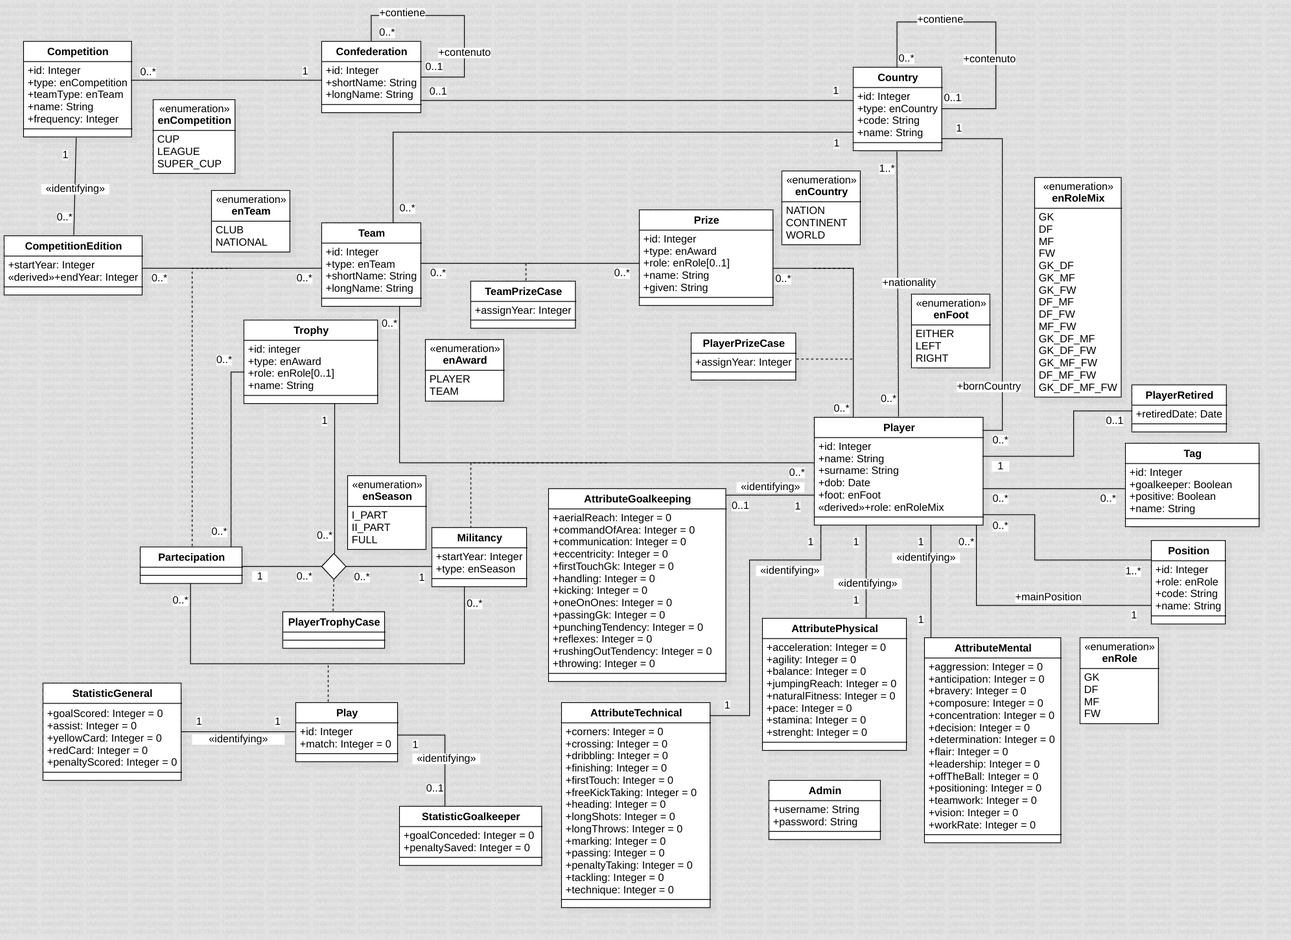
\includegraphics[width=\textwidth]{res/DOC_DATABASE/class_diagram_ristr}
\newpage

\subsection{Dizionario}

\subsection{Dizionario delle Enumerazioni}

\begin{tblr}{
	 hlines = {0.9pt}, vlines = {0.9pt}, colspec = {X[l]X[l]X[l]}, column{1-2}= {110pt},
    width = \textwidth, cell{1}{1-3} = {blue!10!white}
}

	{
		Enumerazione
	}
	&
	{
		Descrizione	
	}
	&
	{
		Litterale
	}
	\\
	{
		\textbf{enAward}
	}
	&
	{
		Rappresenta le possibili tipologie di trofeo e
		premio calcistico.
	}
	&
	{
		\textbf{PLAYER}: Rappresenta un trofeo o premio calcistico
			riferito ad un calciatore.\\
		\medskip\textbf{TEAM}: Rappresenta un trofeo o premio calcistico
			riferito ad una squadra di calcio.
	}
	\\
	{
		\textbf{enCompetition}
	}
	&
	{
		Rappresenta le possibili tipologie di competizione calcistica.
	}
	&
	{
		\textbf{CUP}: Rappresenta le competizioni calcistiche di tipo
			torneo e coppe nazionali.\\
		\medskip\textbf{LEAGUE}: Rappresenta le competizioni calcistiche
			di tipo campionato.\\
		\medskip\textbf{SUPER\_CUP}: Rappresenta le competizioni calcistiche
			di tipo supercoppa.
	}
	\\
	{
		\textbf{enCountry}
	}
	&
	{
		Rappresenta le possibili tipologie di paesi.
	}
	&
	{
		\textbf{NATION}: Rappresenta i paesi di tipo nazione.\\
		\medskip\textbf{CONTINENT}: Rappresenta i paesi di tipo continente.\\
		\medskip\textbf{WORLD}: Rappresenta i paesi di tipo mondo.
	}
	\\
	{
		\textbf{enFoot}
	}
	&
	{
		Rappresenta le possibili tipologie di piede preferito
		di un calciatore.
	}
	&
	{
		\textbf{EITHER}: Rappresenta che il calciatore ha come piede
			preferito, entrambi i piedi.\\
		\medskip\textbf{LEFT}: Rappresenta che il calciatore ha come piede
			preferito, il piede sinistro.\\
		\medskip\textbf{RIGHT}: Rappresenta che il calciatore ha come piede
			preferito, il piede destro.
	}
	\\
	{
		\textbf{enRole}
	}
	&
	{
		Rappresenta le possibili tipologie di ruolo di gioco
		di un calciatore.
	}
	&
	{
		\textbf{GK}: Rappresenta un calciatore che ha
			come ruolo di gioco, il ruolo portiere.\\
		\medskip\textbf{DF}: Rappresenta un calciatore che ha
			come ruolo di gioco, il ruolo difensore.\\
		\medskip\textbf{MF}: Rappresenta un calciatore che ha
			come ruolo di gioco, il ruolo centrocampista.\\
		\medskip\textbf{FW}: Rappresenta un calciatore che ha
			come ruolo di gioco, il ruolo attaccante.
	}
	\\
\end{tblr}

\newpage

\begin{tblr}{
	hlines = {0.9pt}, vlines = {0.9pt}, colspec = {X[l]X[l]X[l]}, column{1-2}= {110pt},
    width = \textwidth
}

	{
		\textbf{enRoleMix}
	}
	&
	{
		Rappresenta tutte le possibili combinazioni di ruolo di gioco
		di un calciatore.
	}
	&
	{
		\textbf{GK}: Rappresenta un calciatore che ha
			come ruolo di gioco, il ruolo portiere.\\
		\medskip\textbf{DF}: Rappresenta un calciatore che ha
			come ruolo di gioco, il ruolo difensore.\\
		\medskip\textbf{MF}: Rappresenta un calciatore che ha
			come ruolo di gioco, il ruolo centrocampista.\\
		\medskip\textbf{FW}: Rappresenta un calciatore che ha
			come ruolo di gioco, il ruolo attaccante.\\
		\medskip\textbf{GK\_DF}: Rappresenta un calciatore che ha
			come ruoli di gioco, il ruolo portiere e il ruolo difensore.\\
		\medskip\textbf{GK\_MF}: Rappresenta un calciatore che ha
			come ruoli di gioco, il ruolo portiere e
			il ruolo centrocampista.\\
		\medskip\textbf{GK\_FW}: Rappresenta un calciatore che ha
			come ruoli di gioco, il ruolo portiere e il ruolo attaccante.\\
		\medskip\textbf{DF\_MF}: Rappresenta un calciatore che ha
			come ruoli di gioco, il ruolo difensore
			e il ruolo centrocampista.\\
		\medskip\textbf{DF\_FW}: Rappresenta un calciatore che ha
			come ruoli di gioco, il ruolo difensore
			e il ruolo attaccante.\\
		\medskip\textbf{MF\_FW}: Rappresenta un calciatore che ha
			come ruoli di gioco, il ruolo centrocampista
			e il ruolo attaccante.\\
		\medskip\textbf{GK\_DF\_MF}: Rappresenta un calciatore che ha
			come ruoli di gioco, il ruolo portiere, il ruolo difensore
			e il ruolo centrocampista.\\
		\medskip\textbf{GK\_DF\_FW}: Rappresenta un calciatore che ha
			come ruoli di gioco, il ruolo portiere, il ruolo difensore
			e il ruolo attaccante.\\
		\medskip\textbf{GK\_MF\_FW}: Rappresenta un calciatore che ha
			come ruoli di gioco, il ruolo portiere, il ruolo centrocampista
			e il ruolo attaccante.\\
		\medskip\textbf{DF\_MF\_FW}: Rappresenta un calciatore che ha
			come ruoli di gioco, il ruolo difensore, il ruolo
			centrocampista e il ruolo attaccante.\\
		\medskip\textbf{GK\_DF\_MF\_FW}: Rappresenta un calciatore che ha
			come ruoli di gioco, il ruolo portiere, il ruolo difensore,
			il ruolo centrocampista e il ruolo attaccante.	
	}
	\\
	{
		\textbf{enSeason}
	}
	&
	{
		Rappresenta le varie tipologie di stagione per una militanza.
	}
	&
	{
		\textbf{I\_PART}: Rappresenta che il calciatore durante la militanza
			ha giocato soltanto nella prima parte di stagione.\\
		\medskip\textbf{II\_PART}: Rappresenta che il calciatore durante
			la militanza ha giocato soltanto nella seconda parte
			di stagione.\\
		\medskip\textbf{FULL}: Rappresenta che il calciatore durante
			la militanza ha giocato per tutta la stagione.
	}
	\\
	{
		\textbf{enTeam}
	}
	&
	{
		Rappresenta le varie tipologie di squadra di calcio.
	}
	&
	{
		\textbf{CLUB}: Rappresenta le squadre di calcio di tipo club.\\
		\medskip\textbf{NATIONAL}: Rappresenta le squadre di calcio di
			tipo nazionale.
	}
	\\
\end{tblr}

\newpage

\subsubsection{Dizionario delle Classi}



\begin{tblr}{
    hlines = {0.9pt}, vlines = {0.9pt}, colspec = {X[l]X[l]X[l]}, column{1-2}= {110pt},
    width = \textwidth, cell{1}{1-3} = {blue!10!white}
}
	{
		Classe
	}
	&
	{
		Descrizione
	}
	&
	{
		Attributo
	}
	\\
	{
		\textbf{Admin}
	}
	&
	{
		Rappresenta gli admin dell'applicativo.
	}
	&
	{
		\textbf{username}(String)[chiave naturale]:\\Rappresenta
			l'username dell'Admin dell'applicativo.\\
		\medskip\textbf{password}(String):\\Rappresenta
			la password dell'Admin dell'applicativo.
	}
	\\
	{
		\textbf{AttributeGoalkeeping}
	}
	&
	{
		Rappresenta gli attributi di un portiere.
	}
	&
	{
		\textbf{aerialReach}(Integer)[default 0]:\\
			Quantifica la capacità fisica di un portiere
			di affrontare situazioni aeree.\\
		\medskip\textbf{commandOfArea}(Integer)[default 0]:\\
			Quantifica la capacità del portiere
			di prendere istintivamente il controllo
			della sua area di rigore.\\
		\medskip\textbf{communication}(Integer)[default 0]:\\
			 Quantifica la capacità del portiere di comunicare
			 con la sua linea difensiva e organizzare
			 il lato difensivo della squadra.\\
		\medskip\textbf{eccentricity}(Integer)[default 0]:\\
			Quantifica la tendenza del portiere
			a fare l'imprevisto, con o senza palla.\\
		\medskip\textbf{firstTouchGk}(Integer)[default 0]:\\
			Quantifica quanto un portiere sia bravo
			a ricevere la palla e a controllarla
			immediatamente quando gli viene passata.\\
		\medskip\textbf{handling}(Integer)[default 0]:\\
			Quantifica la capacità del portiere
			di trattenere la palla quando effettua una parata.\\
		\medskip\textbf{kicking}(Integer)[default 0]:\\
			Quantifica sia la distanza che
			il portiere può calciare e la precisione che
			può trovare sia dai rilanci a mano che
			dalle ripartenza da palla ferma.\\
		\medskip\textbf{oneOnOnes}(Integer)[default 0]:\\
			Quantifica la capacità del portiere
			di fare bene quando si trova
			di fronte a un avversario in una situazione
			di uno contro uno.\\
		\medskip\textbf{passingGk}(Integer)[default 0]:\\
			Quantifica la capacità di un portiere di trovare
			con successo un compagno di squadra con il pallone,
			e la bravura di un portiere nel passare il pallone.\\
		\medskip\textbf{punchingTendency}(Integer)[default 0]:\\
			Quantifica l'inclinazione del portiere
			a respingere il pallone in situazioni
			in cui potrebbe forse tentare di afferrarlo.\\
		\medskip\textbf{reflexes}(Integer)[default 0]:\\
			Quantifica la capacità del portiere
			di reagire a eventi imprevedibili con
			un alto tasso di successo.\\
		\medskip\textbf{rushingOutTendency}(Integer)[default 0]:\\
			Quantifica la tendenza del portiere a uscire
			dalla propria posizione per reagire
			a passaggi filtranti e cross.\\
		\medskip\textbf{throwing}(Integer)[default 0]:\\
			Quantifica la capacità del portiere di lanciare
			con precisione il pallone con le sue mani.
	}
	\\
\end{tblr}

\newpage



\begin{tblr}{
    hlines = {0.9pt}, vlines = {0.9pt}, colspec = {X[l]X[l]X[l]}, column{1-2}= {110pt},
    width = \textwidth
}
	{
		\textbf{AttributeMental}
	}
	&
	{
		Rappresenta gli attributi mentali di un calciatore.
	}
	&
	{
		\textbf{aggression}(Integer)[default 0]:\\
			Quantifica l'atteggiamento di un calciatore
			in termini di mentalità di gioco, ma
			non necessariamente indica
			una tendenza alla scorrettezza.\\
		\medskip\textbf{anticipation}(Integer)[default 0]:\\
			 Quantifica la capacità di un calciatore a prevedere
			 e reagire a un evento.\\
		\medskip\textbf{bravery}(Integer)[default 0]:\\
			Quantifica principalmente quanto il calciatore
			sia dedicato sul campo.\\
		\medskip\textbf{composure}(Integer)[default 0]:\\
			Quantifica la tranquillità mentale del calciatore
			e la sua capacità, in particolare con il pallone
			ma anche senza di esso, di prendere decisioni
			più intelligenti.\\
		\medskip\textbf{concentration}(Integer)[default 0]:\\
			Quantifica la concentrazione mentale di un calciatore
			e l'attenzione ai dettagli su base evento per evento,
			dove i calciatori con alta concentrazione
			saranno in grado di concentrarsi meglio
			per un tempo più lungo e rispondere agli incidenti
			sia precocemente che tardi nella partita.\\
		\medskip\textbf{decision}(Integer)[default 0]:\\
			Quantifica la capacità di un calciatore
			di fare la scelta corretta, sia con
			che senza il pallone,
			nella maggior parte dei casi.\\
		\medskip\textbf{determination}(Integer)[default 0]:\\
			Quantifica l'impegno e la determinazione
			di un calciatore nel voler avere successo
			sia dentro che fuori dal campo.\\
		\medskip\textbf{flair}(Integer)[default 0]:\\
			Quantifica il talento naturale del calciatore
			nel essere creativo e occasionalmente imprevedibile.\\
		\medskip\textbf{leadership}(Integer)[default 0]:\\
			Quantifica la capacità di un calciatore
			di influenzare gli altri calciatori
			intorno a lui sul campo.\\
		\medskip\textbf{offTheBall}(Integer)[default 0]:\\
			Quantifica la capacità di un calciatore
			di muoversi quando non è in possesso della palla,
			rendendosi disponibile per ricevere un passaggio
			in una posizione più pericolosa.\\
		\medskip\textbf{positioning}(Integer)[default 0]:\\
			Quantifica la capacità di un calciatore di leggere
			le situazioni e posizionarsi di conseguenza
			nel modo migliore possibile per affrontare
			gli eventi in corso.\\
		\medskip\textbf{teamwork}(Integer)[default 0]:\\
			Quantifica la capacità di un calciatore
			di seguire le istruzioni tattiche
			mentre lavora per e insieme
			ai suoi compagni di squadra.\\
		\medskip\textbf{vision}(Integer)[default 0]:\\
			Quantifica la capacità di un calciatore
			di individuare una potenziale opportunità.\\
		\medskip\textbf{workRate}(Integer)[default 0]:\\
			Quantifica la determinazione mentale del calciatore
			nel lavorare al massimo delle proprie capacità.
	}
	\\
\end{tblr}

\newpage

\begin{tblr}{
    hlines = {0.9pt}, vlines = {0.9pt}, colspec = {X[l]X[l]X[l]}, column{1-2}= {110pt},
    width = \textwidth
}
	{
		\textbf{AttributePhysical}
	}
	&
	{
		Rappresenta gli attributi fisici di un calciatore.
	}
	&
	{
		\textbf{acceleration}(Integer)[default 0]:\\
			Quantifica quanto rapidamente il calciatore
			raggiunge la massima velocità
			da una posizione di partenza ferma.\\
		\medskip\textbf{agility}(Integer)[default 0]:\\
			Quantifica la capacità di un calciatore di iniziare,
			fermarsi e muoversi in diverse direzioni
			a vari livelli di velocità,
			sia con che senza il pallone.\\
		\medskip\textbf{balance}(Integer)[default 0]:\\
			Quantifica la capacità di un calciatore
			di mantenere l'equilibrio e rimanere in piedi
			con e senza il pallone, controllando
			le proprie azioni durante il movimento,
			un giro di scatto o il cambio di direzione.\\
		\medskip\textbf{jumpingReach}(Integer)[default 0]:\\
			Quantifica la capacità di un calciatore
			di raggiungere il pallone in aria.\\
		\medskip\textbf{naturalFitness}(Integer)[default 0]:\\
			Non è un attributo tipico in relazione
			ad una capacità sul campo di un calciatore,
			ma quantifica piuttosto i suoi geni e
			il livello di forma fisica.\\
		\medskip\textbf{pace}(Integer)[default 0]:\\
			Quantifica la massima velocità di un calciatore.\\
		\medskip\textbf{stamina}(Integer)[default 0]:\\
			Quantifica la capacità di un calciatore
			di sopportare attività fisiche
			ad alto livello per un lungo periodo di tempo.\\
		\medskip\textbf{strenght}(Integer)[default 0]:\\
			Quantifica la capacità di un calciatore
			di esercitare la propria forza fisica
			su un avversario a proprio vantaggio.
	}
	\\
\end{tblr}

\newpage


\begin{tblr}{
    hlines = {0.9pt}, vlines = {0.9pt}, colspec = {X[l]X[l]X[l]}, column{1-2}= {110pt},
    width = \textwidth
}

	{
		\textbf{AttributeTechnical}
	}
	&
	{
		Rappresenta gli attributi tecnici di un calciatore.
	}
	&
	{
		\textbf{corners}(Integer)[default 0]:\\
			Quantifica la capacità di un calciatore
			di eseguire un calcio d'angolo con precisione.\\
		\medskip\textbf{crossing}(Integer)[default 0]:\\
			Quantifica la capacità di un calciatore
			nel calciare il pallone, principalmente
			ma non esclusivamente, dalle aree laterali
			con precisione.\\
		\medskip\textbf{dribbling}(Integer)[default 0]:\\
			Quantifica la capacità di un calciatore
			di correre con il pallone e manipolarlo
			sotto stretto controllo.\\
		\medskip\textbf{finishing}(Integer)[default 0]:\\
			Quantifica la capacità di un calciatore
			di segnare quando gli viene presentata
			un'opportunità.\\
		\medskip\textbf{firstTouch}(Integer)[default 0]:\\
			Quantifica quanto un calciatore sia bravo
			a ricevere la palla e a controllarla
			immediatamente quando gli viene passata.\\ 
		\medskip\textbf{freeKickTaking}(Integer)[default 0]:\\
			Quantifica la capacità di un calciatore
			nel calciare una palla ferma.\\
		\medskip\textbf{heading}(Integer)[default 0]:\\
			Quantifica esclusivamente la capacità
			di un calciatore nel colpire il pallone
			con la testa e nel gestire le situazioni aeree.\\
		\medskip\textbf{longShots}(Integer)[default 0]:\\
			Quantifica la capacità di un giocatore
			nel tirare da distanza, o più precisamente
			dall'esterno dell'area di rigore.\\
		\medskip\textbf{longThrows}(Integer)[default 0]:\\
			Quantifica la capacità di un calciatore di eseguire
			un lancio lungo, che può essere vantaggioso
			nelle situazioni di attacco o per far uscire
			la palla dalle zone difensive e
			portarla più rapidamente nell'ultimo
			terzo del campo.\\
		\medskip\textbf{marking}(Integer)[default 0]:\\
			Quantifica la capacità di un calciatore
			di restare vicino alla sua diretta opposizione
			nelle situazioni difensive.\\
		\medskip\textbf{passing}(Integer)[default 0]:\\
			Quantifica la capacità di un calciatore di trovare
			con successo un compagno di squadra con il pallone,
			e la bravura di un calciatore nel passare il pallone.\\
		\medskip\textbf{penaltyTaking}(Integer)[default 0]:\\
			Quantifica la capacità di un calciatore
			dal dischetto del rigore e determina
			il successo e il fallimento del calcio di rigore.\\
		\medskip\textbf{tackling}(Integer)[default 0]:\\
			Quantifica la capacità di un calciatore nel vincere
			il pallone pulitamente, senza commettere falli,
			quando affronta un altro calciatore.\\
		\medskip\textbf{technique}(Integer)[default 0]:\\
			Quantifica la raffinatezza di un calciatore con
			il pallone - la loro qualità estetica con il pallone,
			sia che si tratti della competenza
			nel passare la palla, nel tirare, nel crossare o
			nel dribblare con il pallone.
	}
	\\
\end{tblr}


\newpage


\begin{tblr}{
    hlines = {0.9pt}, vlines = {0.9pt}, colspec = {X[l]X[l]X[l]}, column{1-2}= {110pt},
    width = \textwidth
}

	{
		\textbf{Competition}
	}
	&
	{
		Rappresenta le competizioni calcistiche.
	}
	&
	{
		\textbf{id}(Integer)[chiave surrogata]:\\Rappresenta
			l'identificativo di una Competizione.\\
		\medskip\textbf{type}(enCompetition):\\Rappresenta
			il tipo di una Competizione.\\
		\medskip\textbf{teamType}(enTeam):\\Rappresenta
			il tipo di squadra che può
			partecipare alla Competizione.\\
		\medskip\textbf{name}(String)[chiave naturale]:
			\\Rappresenta il nome di una Competizione.\\
		\medskip\textbf{frequency}(Integer):\\Rappresenta
			la frequenza di una Competizione.
	}
	\\
	{
		\textbf{CompetitionEdition}
	}
	&
	{
		Rappresenta le edizioni delle competizioni calcistiche.
	}
	&
	{
		\textbf{startYear}(Integer)[chiave parziale]:
			\\Rappresenta l'anno di inizio di un'Edizione.\\
		\medskip\textbf{endYear}(Integer)[derivato]:
			\\Rappresenta l'anno di fine di un'Edizione.
	}
	\\
	{
		\textbf{Confederation}
	}
	&
	{
	Rappresenta le confederazioni calcistiche.
	}
	& 
	{
		\textbf{id}(Integer)[chiave surrogata]:\\Rappresenta
			l'identificativo di una Confederazione.\\
		\medskip\textbf{shortName}(String):\\Rappresenta
			il nome abbreviato di una Confederazione.\\
		\medskip\textbf{longName}(String)[chiave naturale]:
			\\Rappresenta il nome esteso di una Confederazione.
	}
	\\
	{
		\textbf{Country}
	}
	&
	{
		Rappresenta i paesi in cui si gioca
		ufficialmente a calcio.
	}
	&
	{
		\textbf{id}(Integer)[chiave surrogata]:\\Rappresenta
			l'identificativo di un Paese.\\
		\medskip\textbf{type}(enCountry):\\Rappresenta
			il tipo di un Paese.\\
		\medskip\textbf{code}(String)[chiave naturale]:
			\\Rappresenta il codice ISO 3166-1 alpha-3
			di un Paese.\\
		\medskip\textbf{name}(String)[chiave naturale]:
			\\Rappresenta il nome di un Paese.
	}
	\\
	{
		\textbf{Player}
	}
	&
	{
		Rappresenta i calciatori.
	}
	&
	{
		\textbf{id}(Integer)[chiave surrogata]:\\Rappresenta
			l'identificativo di un Calciatore.\\
		\medskip\textbf{name}(String):\\Rappresenta
			il nome di un Calciatore.\\
		\medskip\textbf{surname}(String):\\Rappresenta
			il cognome di un Calciatore.\\
		\medskip\textbf{dob}(Date):\\Rappresenta
			la data di nascita.\\
		\medskip\textbf{foot}(enFoot):\\Rappresenta
			il piede preferito di un Calciatore.\\
		\medskip\textbf{role}(enRoleMix)[derivato]:
			\\Rappresenta i possibili ruoli di gioco
			di un Calciatore.
	}
	\\
\end{tblr}


\newpage


\begin{tblr}{
    hlines = {0.9pt}, vlines = {0.9pt}, colspec = {X[l]X[l]X[l]}, column{1-2}= {110pt},
    width = \textwidth
}

	{
		\textbf{PlayerRetired}
	}
	&
	{
		Rappresenta i calciatori che sono ritirati.
	}
	&
	{
		\textbf{retiredDate}(Date):\\Rappresenta
			la data di ritiro di un calciatore.
	}
	\\
	{
		\textbf{Position}
	}
	&
	{
		Rappresenta le posizioni di gioco di un calciatore.
	}
	&
	{
		\textbf{id}(Integer)[chiave surrogata]:\\Rappresenta
			l'identificativo di una Posizione.\\
		\medskip\textbf{role}(enRole):\\Rappresenta
			il ruolo associato ad una Posizione.\\
		\medskip\textbf{code}(String)[chiave naturale]:
			\\Rappresenta il nome abbreviato di una Posizione.\\
		\medskip\textbf{name}(String)[chiave naturale]:
			\\Rappresenta il nome di una Posizione.
	}
	\\
	{
		\textbf{Prize}
	}
	&
	{
		Rappresenta i premi calcistici.
	}
	&
	{
		\textbf{id}(Integer)[chiave surrogata]:\\Rappresenta
			l'identificativo del Premio.\\
		\medskip\textbf{type}(enAward):\\Rappresenta
			il tipo del Premio.\\
		\medskip\textbf{role}(enRole)[parziale]:\\Rappresenta
			il ruolo a cui è associato un Premio.\\
		\medskip\textbf{name}(String)[chiave naturale]:
			\\Rappresenta il nome del Premio.\\
		\medskip\textbf{given}(String):\\Rappresenta
			il nome della società calcistica
			che conferisce il Premio.
	}
	\\
	{
		\textbf{StatisticGeneral}
	}
	&
	{
		Rappresenta le statistiche generali di un calciatore.
	}
	&
	{
		\textbf{goalScored}(Integer)[default 0]:\\
			Rappresenta il numero di goal segnati
			da un calciatore.\\
		\medskip\textbf{assist}(Integer)[default 0]:\\
			Rappresenta il numero di assist di un calciatore.\\
		\medskip\textbf{yellowCard}(Integer)[default 0]:\\
			Rappresenta il numero di cartellini gialli
			presi da un calciatore.\\
		\medskip\textbf{redCard}(Integer)[default 0]:\\
			Rappresenta il numero di cartellini rossi
			presi da un calciatore.\\
		\medskip\textbf{penaltyScored}(Integer)[default 0]:\\
			Rappresenta il numero di rigori segnati
			da un calciatore.
	}
	\\
	{
		\textbf{StatisticGoalkeeper}
	}
	&
	{
		Rappresenta le statistiche di un portiere.
	}
	&
	{
		\textbf{goalConceded}(Integer)[default 0]:\\
			Rappresenta il numero di goal subiti
			da un portiere.\\
		\medskip\textbf{penaltySaved}(Integer)[default 0]:\\
			Rappresenta il numero di rigori parati
			da un portiere.
	}
	\\
	{
		\textbf{Tag}
	}
	&
	{
		Rappresenta i tag di un calciatore.
	}
	&
	{
		\textbf{id}(Integer)[chiave surrogata]:\\Rappresenta
			l'identificativo del Tag.\\
		\medskip\textbf{goalkeeper}(Boolean):\\
			Rappresenta se un tag è per un portiere oppure no.\\
		\medskip\textbf{positive}(Boolean):\\
			Rappresenta se un tag indica una specialità
			di un calciatore o un suo difetto.\\
		\medskip\textbf{name}(String)[chiave naturale]:
			\\Rappresenta il nome del Tag.
	}
	\\
\end{tblr}

\newpage

\begin{tblr}{
    hlines = {0.9pt}, vlines = {0.9pt}, colspec = {X[l]X[l]X[l]}, column{1-2}= {110pt},
    width = \textwidth
}

	{
		\textbf{Team}
	}
	&
	{
		Rappresenta le squadre di calcio.
	}
	&
	{
		\textbf{id}(Integer)[chiave surrogata]:\\Rappresenta
			l'identificativo della Squadra.\\
		\medskip\textbf{type}(enTeam):\\Rappresenta
			il tipo della Squadra.\\
		\medskip\textbf{shortName}(String):\\
			Rappresenta il nome abbreviato della Squadra.\\
		\medskip\textbf{longName}(String)[chiave naturale]:
			\\Rappresenta il nome esteso della Squadra.
	}
	\\
	{
		\textbf{Trophy}
	}
	&
	{
		Rappresenta i trofei calcistici.
	}
	&
	{
		\textbf{id}(Integer)[chiave surrogata]:\\Rappresenta
			l'identificativo del Trofeo.\\
		\medskip\textbf{type}(enAward):\\Rappresenta
			il tipo del Trofeo.\\
		\medskip\textbf{role}(enRole)[parziale]:\\Rappresenta
			il ruolo a cui è associato un Trofeo.\\
		\medskip\textbf{name}(String)[chiave naturale]:
			\\Rappresenta il nome del Trofeo.
	}
	\\
\end{tblr}

\newpage

\subsubsection{Dizionario delle Associazioni}



\begin{tblr}{
    hlines = {0.9pt}, vlines = {0.9pt}, colspec = {X[l]X[l]X[l]X[l]}, column{1-2}= {100pt},
    width = \textwidth, cell{1}{1-4} = {blue!10!white}
}

	{
		Nome
	}
	&
	{
		Descrizione
	}
	&
	{
		Classe in Relazione
	}
	&
	{
		Attributo
	}
	\\
	{
		\textbf{bornCountry}
	}
	&
	{
		Esprime il paese di nascita di un calciatore.
	}
	&
	{
		\textbf{Country [0 ... *]}:\\Indica che
			uno stesso paese può essere il paese di nascita
			di più calciatori.\\
		\medskip\textbf{Player [1]}:\\Indica che
			un calciatore ha uno e un solo paese di nascita.
	}
	&
	{
	
	}
	\\
	{
		\textbf{Competition-CompetitionEdition}
	}
	&
	{
		Esprime le edizioni di una competizione.\\
		È un'associazione identificante.
	}
	&
	{
		\textbf{Competition[0 ... *]}:\\Indica che
			una Competizione può essere associata
			a più Edizioni.\\
		\medskip\textbf{CompetitionEdition[1]}:\\Indica che
			un'Edizione può essere associata ad una
			e una sola Competizione.
	}
	&
	{
		
	}
	\\
	{
		\textbf{Competition-Confederation}
	}
	&
	{
		Esprime la confederazione che organizza
		la competizione.
	}
	&
	{
		\textbf{Competition [1]}:\\Indica che
			una Competizione può essere associata ad una
			e una sola Confederazione.\\
		\medskip\textbf{Confederation [0 ... *]}:\\Indica che
			una Confederazione può essere associata
			a più Competizioni.	
	}
	&
	{
		
	}
	\\
	{
		\textbf{Confederation-Confederation}
	}
	&
	{
		Esprime la possibilità di una confederazione di
		avere come membri altre confederazioni, o essere
		membro a sua volta.
	}
	&
	{
		\textbf{Confederation [0 ... 1] ruolo (contenuto)}:\\
			Indica che una Confederazione può o non può essere
			membra di un'altra Confederazione.\\
		\medskip\textbf{Confederation [0 ... *]
			ruolo (contiene)}:\\
			Indica che una Confederazione può contenere
			più Confederazioni.
	}
	&
	{
		
	}
	\\
	{
		\textbf{Confederation-Country}
	}
	&
	{
		Esprime l'appartenza di una confederazione
		ad un unico paese.
	}
	&
	{
		\textbf{Confederation [1]}:\\Indica che
			una Confederazione può essere associata
			ad un e un solo Paese.\\
		\medskip\textbf{Country [0 ... 1]}:\\Indica che
			un Paese può essere associato a nessuna o
			ad una Confederazione.
	}
	&
	{
		
	}
	\\
\end{tblr}

\newpage

\begin{tblr}{
    hlines = {0.9pt}, vlines = {0.9pt}, colspec = {X[l]X[l]X[l]X[l]}, column{1-2}= {90pt},
    width = \textwidth
}

	{
		\textbf{Country-Country}
	}
	&
	{
		Esprime la possibilità di un paese di
		essere contenuto geograficamente in un altro paese,
		oppure di contenere paesi.
	}
	&
	{
		\textbf{Country [0 ... 1] ruolo (contenuto)}:\\
			Indica che un Paese può o non può essere
			geograficamente contenuto in un altro Paese.\\
		\medskip\textbf{Country [0 ... *]
			ruolo (contiene)}:\\
			Indica che un Paese può contenere
			più paesi.
	}
	&
	{
		
	}
	\\
	{
		\textbf{MainPosition}
	}
	&
	{
		Esprime la posizione principale di un calciatore.
	}
	&
	{
		\textbf{Player [1]}:\\Indica che un calciatore
			ha una e una sola posizione principale.\\
		\medskip\textbf{Position [0 ... *]}:\\Indica che
			una stessa posizione può essere la posizione principale
			di più calciatori.
	}
	&
	{
	
	}
	\\
	{
		\textbf{Militancy}
	}
	&
	{
		Esprime le militanze di un calciatore in una squadra
		per stagione.
	}
	&
	{
		\textbf{Player [0 ... *]}:\\Indica che un Calciatore
			può militare in più Squadre.\\
		\medskip\textbf{Team [0 ... *]}:\\Indica che una Squadra
			può essere associata a più Calciatori.
	}
	&
	{
		\textbf{startYear}(Integer):\\Rappresenta
			la stagione di riferimento di una Militanza.\\
		\medskip\textbf{type}(enSeason):\\Rappresenta
			fino a che parte della stagione un Calciatore
			militava per quella Squadra.
	}
	\\
	{
		\textbf{Nationality}
	}
	&
	{
		Esprime le nazionalità di un calciatore.
	}
	&
	{
		\textbf{Country [0 ... *]}:\\Indica che
			uno stesso paese può essere associato a più
			calciatore.\\
		\medskip\textbf{Player [1 ... *]}:\\Indica che
			un calciatore ha una o più nazionalità.
	}
	&
	{
	
	}
	\\
	{
		\textbf{Partecipation}
	}
	&
	{
		Esprime  la partecipazione di una squadra
		ad un'edizione di una competizione.
	}
	&
	{
		\textbf{Team [0 ... *]}:\\Indica che una Squadra
			può partecipare a più Edizioni.\\
		\medskip\textbf{CompetitionEdition [0 ... *]}:
			\\Indica che una Edizione può essere associata
			a più squadre.

	}
	&
	{
		
	}
	\\
	{
		\textbf{Partecipation-Trophy}
	}
	&
	{
		Esprime la bacheca dei trofei di una squadra.
	}
	&
	{
		\textbf{Trophy [0 ... *]}:\\Indica che un Trofeo
			può essere associata a più Partecipazioni
			di una Squadra ad una Edizione.\\
		\medskip\textbf{Partecipation [0 ... *]}:\\Indica che
			una Partecipazione può essere associata
			a più Trofei.
	}
	&
	{
		
	}
	\\
\end{tblr}

\newpage

\begin{tblr}{
    hlines = {0.9pt}, vlines = {0.9pt}, colspec = {X[l]X[l]X[l]X[l]}, column{1-2}= {105pt},
    width = \textwidth
}

	{
		\textbf{Play}
	}
	&
	{
		Esprime in quale edizione di una competizione
		un calciatore, che militava per una certa squadra,
		ha giocato.
	}
	&
	{
		\textbf{Partecipation [0 ... *]}:\\Indica che
			una Partecipazione può essere associata
			a più Rose.\\
		\medskip\textbf{Militancy [0 ... *]}:\\Indica che
			una Militanza può essere associata
			a più Partecipazioni.
	}
	&
	{
		\textbf{id}(Integer)[chiave surrogata]:\\Rappresenta
			l'identificativo di un Gioco.\\
		\medskip\textbf{match}(Integer):\\Rappresenta
			il numero di presenze di un calciatore
			in un Gioco.
	}
	\\
	{
		\textbf{Play-StatisticGeneral}
	}
	&
	{
		Esprime le stastistiche generali di un calciatore
		per un gioco.\\È un'associazione identificante.
	}
	&
	{
		\textbf{Play [1]}:\\Indica che un Gioco si riferisce
			ad uno e una sola Statistica generale.\\
		\medskip\textbf{StatisticGeneral [1]}:\\Indica che
			una Statistica generale si riferisce
			ad un e un solo Gioco.
	}
	&
	{
		
	}
	\\
	{
		\textbf{Play-StatisticGoalkeeper}
	}
	&
	{
		Esprime le statistiche di un portiere per un gioco.\\
		È un'associazione identificante.
	}
	&
	{
		\textbf{Play [0 ... 1]}:\\Indica che un Gioco può
			essere o non essere associato alle Statistiche
			per portieri.\\
		\medskip\textbf{StatisticGoalKeeper[1]}:\\Indica che
			una Statistica per portieri si riferisce
			ad un e un solo Gioco.
	}
	&
	{
		
	}
	\\
	{
		\textbf{Player-AttributeGoalkeeping}
	}
	&
	{
		Esprime i calciatori associati agli
		attributi dei portieri.\\È un'associazione identificante.
	}
	&
	{
		\textbf{Player [0 ... 1]}:\\Indica che un Calciatore
			può essere o non essere associato ad un Attributo
			dei portieri.\\
		\medskip\textbf{AttributeGoalkeeping [1]}:\\Indica che
			un Attributo dei portieri si riferisce
			ad un e un solo Calciatore.
	}
	&
	{
		
	}
	\\
	{
		\textbf{Player-AttributeMental}
	}
	&
	{
		Esprime i calciatori associati ad un Attributo mentale.\\
		È un'associazione identificante.
	}
	&
	{
		\textbf{Player [1]}:\\Indica che un Calciatore
			si riferisce ad un e un solo Attributo mentale.\\
		\medskip\textbf{AttributeMental [1]}:\\Indica che
			un Attributo mentale si riferisce ad un
			e un solo Calciatore.
	}
	&
	{
	
	}
	\\
	{
		\textbf{Player-AttributePhysical}
	}
	&
	{
		Esprime i calciatori associati ad un Attributo fisico.\\
		È un'associazione identificante.
	}
	&
	{
		\textbf{Player [1]}:\\Indica che un Calciatore
			si riferisce ad un e un solo Attributo fisico.\\
		\medskip\textbf{AttributePhysical [1]}:\\Indica che
			un Attributo fisico si riferisce ad un
			e un solo Calciatore.
	}
	&
	{
		
	}
	\\
\end{tblr}

\newpage

\begin{tblr}{
    hlines = {0.9pt}, vlines = {0.9pt}, colspec = {X[l]X[l]X[l]X[l]}, column{1-2}= {100pt},
    width = \textwidth
}

	{
		\textbf{Player-AttributeTechnical}
	}
	&
	{
		Esprime i calciatori associati ad un Attributo tecnico.\\
		È un'associazione identificante.
	}
	&
	{
		\textbf{Player [1]}:\\Indica che un Calciatore
			si riferisce ad un e un solo Attributo tecnico.\\
		\medskip\textbf{AttributeTechnical [1]}:\\Indica che
			un Attributo tecnico si riferisce ad un
			e un solo Calciatore.
	}
	&
	{
		
	}
	\\
	{
		\textbf{Player-PlayerRetired}
	}
	&
	{
		Esprime i calciatori ritirati.
	}
	&
	{
		\textbf{Player [0 ... 1]}:\\Indica che
			un Calciatore può essere o non essere ritirato.\\
		\medskip\textbf{PlayerRetired [1]}:\\Indica che
			una data di ritiro si riferisce ad uno
			e un solo Calciatore. 
	}
	&
	{
	
	}
	\\
	{
		\textbf{Player-Position}
	}
	&
	{
		Esprime le posizioni di gioco di un calciatore.
	}
	&
	{
		\textbf{Player [1 ... *]}:\\Indica che
			un Calciatore può essere associato
			a una o più Posizioni.\\
		\medskip\textbf{Position [0 ... *]}:\\Indica che
			una Posizione può essere associata a più Calciatori.
	}
	&
	{
		
	}
	\\
	{
		\textbf{PlayerPrizeCase}
	}
	&
	{
		Esprime i premi di un calciatore.
	}
	&
	{
		\textbf{Player [0 ... *]}:\\Indica che
			un Calciatore può essere associato a più Premi.\\
		\medskip\textbf{Prize [0 ... *]}:\\Indica che
			un Premio può essere associato, in anni diversi,
			a più Premi.
				
	}
	&
	{
		\textbf{assignYear}(Integer):\\Rappresenta
			l'anno di assegnazione del Premio al Calciatore.
	}
	\\
	{
		\textbf{Player-Tag}
	}
	&
	{
		Esprime i tag di un calciatore.
	}
	&
	{
		\textbf{Player [0 ... *]}:\\Indica che
			un Calciatore può essere associato a più Tag.\\
		\medskip\textbf{Tag [0 ... *]}:\\Indica che
			uno Tag può essere associato a più Calciatori.
	}
	&
	{
		
	}
	\\
\end{tblr}


\newpage

\begin{tblr}{
    hlines = {0.9pt}, vlines = {0.9pt}, colspec = {X[l]X[l]X[l]X[l]}, column{1-2}= {100pt},
    width = \textwidth
}

	{
		\textbf{PlayerTrophyCase}	
	}
	&
	{
		Esprime la bacheca dei trofei di un calciatore.
	}
	&
	{
		\textbf{Partecipation [0 ... *]}:\\Indica che
			una Partecipazione può essere associata
			a più Bacheche.\\
		\medskip\textbf{Trophy [0 ... *]}:\\Indica che
			un Trofeo può essere associato
			a più Bacheche.\\
		\medskip\textbf{Militancy [0 ... *]}:\\Indica che
			una Militanza può essere associata
			a più Bacheche.\\
		\medskip\textbf{PlayTrophyCase -> Partecipation [1]}:
			\\Indica che una Bacheca può essere associata
			ad una e una sola Partecipazione.\\
		\medskip\textbf{PlayTrophyCase -> Trophy [1]}:
			\\Indica che una Bacheca può essere associata
			ad un e un solo Trofeo.\\
		\medskip\textbf{PlayTrophyCase -> Militancy [1]}:
			\\Indica che una Bacheca può essere associata
			ad una e una sola Militanza.
	}
	&
	{
		
	}
	\\
	{
		\textbf{Team-Country}
	}
	&
	{
		Esprime la nazionalità di una squadra.
	}
	&
	{
		\textbf{Team [1]}:\\Indica che una Squadra
			può essere associata ad un e un solo Paese.\\
		\medskip\textbf{Country [0 ... *]}:\\Indica che
			un Paese può essere associato a più Squadre.	
	}
	&
	{
		
	}
	\\
	{
		\textbf{TeamPrizeCase}
	}
	&
	{
		Esprime i premi di una squadra.
	}
	&
	{
		\textbf{Team [0 ... *]}:\\Indica che
			una Squadra può essere associata a più Premi.\\
		\medskip\textbf{Prize [0 ... *]}:\\Indica che
			un Premio, in anni diversi, a più Squadre.
	}
	&
	{
		\textbf{assignYear}(Integer):\\Rappresenta
			l'anno di assegnazione di un Premio ad una Squadra.\\
	}
	\\
\end{tblr}

\newpage

\subsubsection{Dizionario dei Vincoli}


\begin{tblr}{
    hlines = {0.9pt}, vlines = {0.9pt}, colspec = {X[l]X[l]X[l]}, 
    width = \textwidth, cell{1}{1-3} = {blue!10!white}, column{2}= {110pt}
}
	{
		Vincolo
	}
	&
	{
		Tipo
	}
	&
	{
		Descrizione
	}
	\\
	{
		\textbf{uqCountryCode}
	}
	&
	{
		INTRARELAZIONALI
	}
	&
	{
		Non possono esistere paesi diversi con
		lo stesso codice.
	}
	\\
	{
		\textbf{uqCountryName}
	}
	&
	{
		INTRARELAZIONALI
	}
	&
	{
		Non possono esistere paesi diversi con
		lo stesso nome.
	}
	\\
	{
		\textbf{ckCountrySuper}
	}
	&
	{
		N-UPLA
	}
	&
	{
		Un paese di tipo mondo non ha un paese che lo contiene.
	}
	\\
	{
		\textbf{Controllo CountryContinent}
	}
	&
	{
		INTRARELAZIONALI
	}
	&
	{
		Il numero di paesi di tipo continente può essere
		al massimo uguale a sette.
	}
	\\
	{
		\textbf{Controllo CountryWorld}
	}
	&
	{
		INTRARELAZIONALI
	}
	&
	{
		Il numero di paesi di tipo mondo può essere
		al massimo uguale a uno.
	}
	\\
	{
		\textbf{Controllo CountrySuper}
	}
	&
	{
		INTRARELAZIONALI
	}
	&
	{
		Un paese deve essere contenuto soltanto in un paese
		con tipo strettamente superiore.\\
		(es. NATION->CONTINENT->WORLD).
	}
	\\
	{
		\textbf{uqConfederationLongName}
	}
	&
	{
		INTRARELAZIONALI
	}
	&
	{
		Non possono esistere confederazioni calcistiche
		diverse con lo stesso nome esteso.
	}
	\\
	{
		\textbf{Controllo ConfederationSuper}
	}
	&
	{
		INTRARELAZIONALI
	}
	&
	{
		Una confederazione deve essere membro soltanto di una
		una confederazione con tipo strettamente superiore.\\
		(es. NATION->CONTINENT->WORLD).
	}
	\\
	{
		\textbf{uqCompetitionName}
	}
	&
	{
		INTRARELAZIONALI
	}
	&
	{
		Non possono esistere competizioni calcistiche
		diverse con lo stesso nome.
	}
	\\
	{
		\textbf{Controllo Comp}
	}
	&
	{
		INTERELAZIONALI
	}
	&
	{
		Una competizione calcistica tra squadre nazionali
		non deve avere associata una confederazione
		di tipo nazionale.
	}
	\\
	{
		\textbf{Controllo CompEdFreq}
	}
	&
	{
		INTERELAZIONALI
	}
	&
	{
		L'anno di inizio di un'edizione di una competizione calcistica,
		deve rispettare la frequenza della sua competizione
		di riferimento.
		
	}
	\\
	{
		\textbf{uqTeam}
	}
	&
	{
		INTRARELAZIONALI
	}
	&
	{
		Non possono esistere squadre di calcio diverse
		con lo stesso nome.
	}
	\\
	{
		\textbf{Controllo TeamCountry}
	}
	&
	{
		INTERELAZIONALI
	}
	&
	{
		Una squadra di calcio deve essere associata soltanto
		ad un paese che sia una nazione.
		
	}
	\\
	{
		\textbf{Controllo TeamNatLongName}
	}
	&
	{
		INTERELAZIONALI
	}
	&
	{
		Una squadra di calcio nazionale deve avere il
		suo nome esteso  uguale al nome del paese associato.
	}
	\\
	{
	
		\textbf{Controllo TeamNatShortName}
	}
	&
	{
		INTERELAZIONALI
	}
	&
	{
		Una squadra di calcio nazionale deve avere il
		suo nome abbreviato uguale al codice del paese associato.
	}
	\\
\end{tblr}

\newpage

\begin{tblr}{
    hlines = {0.9pt}, vlines = {0.9pt}, colspec = {X[l]X[l]X[l]}, 
    width = \textwidth, column{2}= {110pt}
}

	{
		\textbf{uqPositionCode}
	}
	&
	{
		INTRARELAZIONALI
	}
	&
	{
		Non possono esistere posizioni di gioco
		diverse con lo stesso codice.
	}
	\\
	{
		\textbf{uqPositionName}
	}
	&
	{
		INTRARELAZIONALI
	}
	&
	{
		Non possono esistere posizioni di gioco
		diverse con lo stesso nome.
	}
	\\
	{
		\textbf{uqPlayer}
	}
	&
	{
		INTRARELAZIONALI	
	}
	&
	{
		Non possono esistere calciatori diversi
		con la stessa combinazione di nome,
		cognome, data di nascita e paese di nascita.
	}
	\\
	{
		\textbf{Controllo PlayerBornNat}
	}
	&
	{
		INTERELAZIONALI
	}
	&
	{
		Un calciatore deve essere associato ad
		un paese di nascita che sia una nazione.
	}
	\\
	{
		\textbf{Controllo PlayerRole}
	}
	&
	{
		N-UPLA
	}
	&
	{
		Un calciatore, al momento dell'inserimento,
		deve avere come valore dell'attributo role
		il valore di role della posizione principale associata.
	}
	\\
	{
		\textbf{Controllo PlayerRetiredDate}
	}
	&
	{
		INTERELAZIONALI
	}
	&
	{
		La sottrazione tra la data di ritiro di un calciatore e
		la sua data di nascita deve essere compresa tra
		l'età minima di un calciatore e l'età massima.
	}
	\\
	{
		\textbf{Controllo PlayerRetiredMilitancy}
	}
	&
	{
		INTERELAZIONALI
	}
	&
	{
		La data di ritiro di un calciatore deve
		essere successiva all'anno d'inizio
		dell'ultima militanza giocata dal calciatore.
	}
	\\
	{
		\textbf{Controllo Nationality}
	}
	&
	{
		INTERELAZIONALI
	}
	&
	{
		Un calciatore ha come nazionalità soltanto
		paesi che siano una nazione.
	}
	\\
	{
		\textbf{Controllo PartTotTeam}
	}
	&
	{
		INTERELAZIONALI
	}
	&
	{
		La partecipazione di una squadra di calcio
		ad un'edizione di una competizione calcistica
		deve essere accettata soltanto se
		il numero massimo di squadre partecipanti per
		quell'edizione non è stato raggiunto.
	}
	\\
	{
		\textbf{uqMilitancy}
	}
	&
	{
		INTRARELAZIONALI
	}
	&
	{
		Un calciatore non può militare nella stessa tipologia
		di squadra di calcio nella stessa parte
		di una stagione calcistica.
	}
	\\
	{
		\textbf{ckMilitancy}
	}
	&
	{
		N-UPLA
	}
	&
	{
		 La militanza per un calciatore in una squadra nazionale
		 deve durare per l'intera stagione in cui è stato convocato.
	}
	\\
	{
		\textbf{Controllo MilitancyValidRange}
	}
	&
	{
		INTERELAZIONALI
	}
	&
	{
		L'anno d'inizio della militanza di un calciatore
		per una squadra di calcio deve essere
		un anno valido per il calciatore.
	}
	\\
	{
		\textbf{Controllo MilitancyTeamNatPlayer}
	}
	&
	{
		INTERELAZIONALI	
	}
	&
	{
		La militanza di un calciatore per
		una squadra di calcio nazionale deve
		essere accettata se il paese associato
		alla squadra di calcio nazionale è una
		nazionalità del calciatore.
	}
	\\
	{
		\textbf{Controllo MilitancyTeamNat}
	}
	&
	{
		INTRARELAZIONALI
	}
	&
	{
		La militanza di un calciatore per
		una squadra di calcio nazionale deve
		essere accettata se il calciatore non ha
		nessun'altra militanza con squadre di calcio nazionali
		diverse da quella considerata.
	}
	\\
\end{tblr}


\newpage


\begin{tblr}{
    hlines = {0.9pt}, vlines = {0.9pt}, colspec = {X[l]X[l]X[l]}, 
    width = \textwidth , column{2}={110pt}
}


	{
		\textbf{Controllo Militancy}
	}
	&
	{
		INTRARELAZIONALI	
	}
	&
	{
		La militanza di un calciatore per
		una squadra di calcio deve essere
		accettata se non vi è una sovrapposizione
		temporale con altre militanze dello
		stesso calciatore per altre squadre di calcio
		dello stesso tipo di quella in considerazione.
	}
	\\
	{
		\textbf{uqPlay}
	}
	&
	{
		INTRARELAZIONALI
	}
	&
	{
		Un calciatore può giocare al più una volta
		per ogni edizione di una competizione calcistica
		in una squadra di calcio.
	}
	\\
	{
		\textbf{Controllo PlayMatchCup}
	}
	&
	{
		INTERELAZIONALI
	}
	&
	{
		Il numero di match di un gioco per un'edizione
		di una competizione di tipo coppa deve essere
		al massimo pari a dieci.
	}
	\\
	{
		\textbf{Controllo PlayMatchLeague}
	}
	&
	{
		INTERELAZIONALI
	}
	&
	{
		Il numero di match di un gioco per un'edizione
		di una competizione di tipo campionato deve essere
		al massimo pari a quaranta.
	}
	\\
	{
		\textbf{Controllo PlayMatchSuperCup}
	}
	&
	{
		INTERELAZIONALI
	}
	&
	{
		Il numero di match di un gioco per un'edizione
		di una competizione di tipo supercoppa deve essere
		al massimo pari a tre.
	}
	\\
	{
		\textbf{uqTagName}
	}
	&
	{
		INTRARELAZIONALI
	}
	&
	{
		Non possono esistere tag diversi con
		lo stesso nome.
	}
	\\
	{
		\textbf{Controllo PlayerTagGK}
	}
	&
	{
		INTERELAZIONALI
	}
	&
	{
		Un Tag per i portieri deve essere associato
		ad un calciatore soltanto se portiere è uno dei
		ruoli in campo del calciatore.
	}
	\\
	{
		\textbf{Controllo AttrGkPlayer}
	}
	&
	{
		INTERELAZIONALI
	}
	&
	{
		Un Attributo per i portieri deve essere associato
		ad un calciatore soltanto se portiere è uno dei
		ruoli in campo del calciatore.
	}
	\\
	{
		\textbf{Controllo StatisticGkPlayer}
	}
	&
	{
		INTERELAZIONALI
	}
	&
	{
		Una Statistica per i portieri deve essere associato
		ad un calciatore soltanto se portiere è uno dei
		ruoli in campo del calciatore.
	}
	\\
	{
		\textbf{uqTrophyName}
	}
	&
	{
		INTRARELAZIONALI
	}
	&
	{
		 Non possono esistere trofei calcistici diversi
		 con lo stesso nome.
	}
	\\
	{
		\textbf{ckTrophy}
	}
	&
	{
		N-UPLA
	}
	&
	{
		I trofei di squadra non devono essere associati
		ad alcun ruolo.
	}
	\\
	{
		\textbf{Controllo TeamTrophyCase}
	}
	&
	{
		INTERELAZIONALI
	}
	&
	{
		Una squadra di calcio deve essere associata
		soltanto a trofei di tipo squadra.
	}
	\\
	{
		\textbf{Controllo PlayerTrophyCaseMil}
	}
	&
	{
		INTERELAZIONALI
	}
	&
	{
		Un trofeo deve essere associato ad 
		un calciatore soltanto se la sua militanza,
		nella stagione in cui è stato vinto il trofeo,
		non è stata per la prima parte.
	}
	\\
	{
		\textbf{Controllo PlayerTrophyCaseTeam}
	}
	&
	{
		INTERELAZIONALI
	}
	&
	{
		Un trofeo di tipo squadra deve essere associato
		ad un calciatore soltanto se la squadra di calcio
		in cui il calciatore militava nella stagione
		di assegnazione del trofeo, ha vinto quel trofeo.
	}
	\\
\end{tblr}

\newpage

\begin{tblr}{
    hlines = {0.9pt}, vlines = {0.9pt}, colspec = {X[l]X[l]X[l]}, 
    width = \textwidth , column{2}={110pt}
}

	{
		\textbf{Controllo PlayerTrophyCaseRole}
	}
	&
	{
		INTERELAZIONALI
	}
	&
	{
		Un trofeo di tipo calciatore
		in uno specifico ruolo deve essere associato
		ad un calciatore soltanto se il ruolo a cui
		è associato il trofeo è un ruolo di gioco
		del calciatore
	}
	\\
	{
		\textbf{uqPrizeName}
	}
	&
	{
		INTRARELAZIONALI
	}
	&
	{
		Non possono esistere premi calcistici diversi
		con lo stesso nome.
	}
	\\
	{
		\textbf{ckPrize}
	}
	&
	{
		N-UPLA
	}
	&
	{
		I premi di squadra non devono essere associati
		ad alcun ruolo.
	}
	\\
	{
		\textbf{Controllo TeamPrize}
	}
	&
	{
		INTERELAZIONALI
	}
	&
	{
		Una squadra di calcio deve essere associata
		soltanto a premi di tipo squadra.
	}
	\\
	{
		\textbf{Controllo PlayerPrize}
	}
	&
	{
		INTERELAZIONALI
	}
	&
	{
		Un calciatore deve essere associato soltanto
		a premi di tipo calciatore.
	}
	\\
	{
		\textbf{Controllo PlayerPrizeValidRange}
	}
	&
	{
		INTERELAZIONALI	
	}
	&
	{
		L'anno di assegnazione di un premio ad
		un calciatore deve essere un anno valido
		del calciatore.
	}
	\\
	{
		\textbf{Controllo PlayerPrizeRole}
	}
	&
	{
		INTERELAZIONALI
	}
	&
	{
		Un premio di tipo calciatore
		in uno specifico ruolo deve essere associato
		ad un calciatore soltanto se il ruolo a cui
		è associato il premio è un ruolo di gioco
		del calciatore.
	}
	\\
	{
		\textbf{dmAlnum}
	}
	&
	{
		DOMINIO
	}
	&
	{
		Dominio per gli attributi delle seguenti classi:\\
		shortName e longName di Confederation;\\
		name di Team;\\
		name di Competition.\\
		Questo dominio sfrutta l' espressione regolare
		che accetta una stringa di caratteri alfanumerici
		(inclusi i caratteri accentati)
		di lunghezza compresa tra i due e i cento caratteri.
		Inoltre, blocca l'inserimento di stringhe
		con ripetizioni di segni di punteggiatura
		e spazi che non siano validi.
	}
	\\
	{
		\textbf{dmAttribute}
	}
	&
	{
		DOMINIO
	}
	&
	{
		Dominio per gli attributi delle classi Attribute.
		Questo dominio permette l'inserimento di
		valori numerici che siano compresi tra zero e dieci.
	}
	\\
	{
		\textbf{dmCode}
	}
	&
	{
		DOMINIO
	}
	&
	{
		Dominio per gli attributi code delle classi:
		country e position.
		Questo dominio sfrutta l'espressione regolare
		che accetta una stringa di caratteri 
		dell'alfabeto inglese maiuscoli di 
		lunghezza compresa tra
		i due e i tre caratteri.
	}
	\\
	{
		\textbf{dmDate}
	}
	&
	{
		DOMINIO
	}
	&
	{
		Dominio per tutti gli attributi di tipo Date.
		Questo dominio permette di inserire date che siano
		precedenti o uguali a quella corrente
		e maggiori o uguali ad una data arbitraria
		che permette l'inserimento di calciatori
		che idealmente giochino la prima stagione
		possibile.
	}
	\\
\end{tblr}


\newpage

\begin{tblr}{
    hlines = {0.9pt}, vlines = {0.9pt}, colspec = {X[l]X[l]X[l]},  column{2}={110pt},
    width = \textwidth
}
	
	{
		\textbf{dmPassword}
	}
	&
	{
		DOMINIO
	}
	&
	{
		Dominio per l'attributo password di UserAccount.
		Questo dominio sfrutta l'espressione regolare
		che accetta una stringa alfanumerica
		di lunghezza compresa tra gli otto e
		i duecentocinquantacinque caratteri.
		Inoltre, è necessaria la presenza
		di almeno una cifra, una lettera maiuscola,
		una lettera minuscola ed un carattere speciale.
	}
	\\
	{
		\textbf{dmString}
	}
	&
	{
		DOMINIO
	}
	&
	{
		Dominio per tutti i restanti attributi
		di tipo	String.
		Questo dominio sfrutta l'espressione regolare
		che accetta una stringa di caratteri
		(inclusi i caratteri accentati)
		di lunghezza compresa tra i due e
		i cento caratteri.
		Inoltre, blocca l'inserimento di stringhe
		con ripetizioni di segni di punteggiatura
		e spazi che non siano validi.
	}
	\\
	{
		\textbf{dmUsername}
	}
	&
	{
		DOMINIO
	}
	&
	{
		Dominio per l'attributo username di UserAccount.
		Questo dominio sfrutta l'espressione regolare
		che accetta una stringa di caratteri alfanumerici
		(inclusi i caratteri accentati), punti,
		trattini e trattini bassi,
		di lunghezza compresa tra i quattro e
		i venti caratteri.
		Inoltre, la stringa non deve iniziare e/o finire
		con punti, trattini e trattini bassi.
		
	}
	\\
	{
		\textbf{dmUsint}
	}
	&
	{
		DOMINIO
	}
	&
	{
		Dominio per tutti i restanti attributi
		di tipo integer.
		Questo dominio non permette di far inserire
		valori numerici inferiori allo zero.
	}
	\\
	{
		\textbf{dmYear}
	}
	&
	{
		DOMINIO
	}
	&
	{
		Dominio per gli attributi year delle classi:
		CompetitionEdition, TeamPrizeCase e
		PlayerPrizeCase.
		Questo dominio permette di inserire anni che siano
		precedenti o uguali a quello corrente
		e maggiori o uguali all'anno in cui è
		ufficialmente nato il calcio.
	}
	\\
\end{tblr}

